\documentclass{article}

\usepackage[utf8x]{inputenc}
\usepackage[english,russian]{babel}
\usepackage{graphicx}
\usepackage{amsmath}
\usepackage{amssymb}
\usepackage{extarrows}
\usepackage{vmargin}
\usepackage{MnSymbol}
\setpapersize{A4}
\setmarginsrb{2cm}{2cm}{2cm}{2cm}{0pt}{0mm}{0pt}{13mm}
%\usepackage{cmap}

\newtheorem{theorem}{Теорема}


\begin{document}

\centerline{\large Курс лекция для магистров ВМК МГУ}
\centerline {\textbf{\LARGE Обратные задачи математической физики}}
\centerline {Затехал Строков Вениамин 2025}

\vspace{0.4cm}

\centerline{\LARGE Лекция 3. Задача определение формы}

\vspace{1cm}
\centerline{\large Единственность}

Рассмотрим класс тел, имеющих средние плоскости, т.е. для них $\exists$ плоскость $P$ такая, что если $Oz \bot P$, то поверхность тела описывается уравнением
\[
z = \varphi(x,y), z = \psi(x,y).
\]

\begin{theorem}
(единственности): \\
При постоянной известной плотности двух тел допустим, что тела обладают параллельными средними плоскостями и центры тяжести расположены внутри тел. Тогда при равенстве внешних потенциалов тела совпадают.
\end{theorem}
Доказательство:

Если
\[
v(M) = \iiint_T \dfrac{\sigma(M')}{z_{MM'}} d \tau_{M'} = 0,
\]
вне тела $T$, то $\sigma \bot \forall$ гармонической функции $u(M)$ в $T$. Действительно, из II формулы Грина имеем:
\[
\iiint_T (\Delta v u - \Delta u v) d \tau = \{\Delta u = 0\} = \iint_{\partial T} [\dfrac{\partial v}{\partial n} u - \dfrac{\partial u}{\partial n} v] ds = 0 = - 4 \pi \iiint \sigma u d\tau.
\]

Рассмотрим тело $T_1 \bigcup T_2$, для $T_1$, $T_2$, имеющих параллельные средние плоскости $z = z_1$ и $z = z_2$.
Тогда $\forall$ гармонической функции $u(M)$ в $T$:
\[
\iiint_{T = T_1 \bigcup T_2} \sigma (M) u(M) d\tau_M = 0 
\]
где
\[
\sigma(M) = 
	\begin{cases}
	1, & M \in T_1 \setminus (T_1 \bigcap T_2);\\
	0, & M \in T_1 \bigcap T_2;\\
	-1, &M \in T_2 \setminus (T_1 \bigcap T_2).
	\end{cases}
\]
т.е. $\sigma (M) = \sigma_1 - \sigma_2$ - разность плотностей.

\vspace{0.5cm}
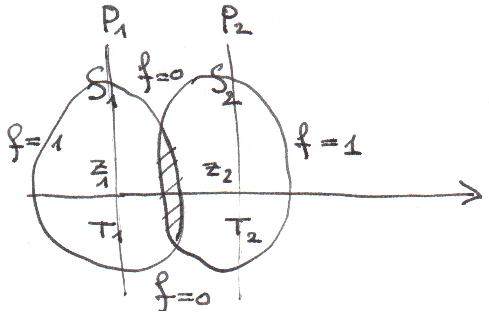
\includegraphics[scale=0.85]{pic1.png}

Рассмотрим 
\[
f(P) = 
	\begin{cases}
	1, & z < z_1, P \in S_1;\\
	1, & z > z_2, P \in S_2;\\
	0, & \text{иначе}.
	\end{cases}
\]
и поставим задачу Дирихле в $T$:
\[
\begin{cases}
\Delta F = 0, & M \in T;\\
F \bigg|_S = f, & S = \partial T.
\end{cases}
\]

Очевидно, что $\dfrac{\partial F}{\partial z}$ гармоническая в $T$. По формуле Остроградского имеем:
\[
\begin{split}
\iiint_T \sigma \dfrac{\partial F}{\partial z} dx dy dz = 
\iiint_{T_1} \sigma_1 \dfrac{\partial F}{\partial z} dx dy dz &- 
\iiint_{T_2} \sigma_2 \dfrac{\partial F}{\partial z} dx dy dz=\\
= - \iint_{S_1} F \bigg|_{z<z_1} dx dy - \iint_{S_2} F \bigg|_{z>z_2} dx dy &+ \iint_{S_1} F \bigg|_{z>z_1} dx dy + \iint_{S_2} F \bigg|_{z<z_2} dx dy = \\
= -f \bigg|_{z<z_1}|s_1| - f \bigg|_{z > z_2} |s_2| &+ F^* \bigg|_{z_>z_1} |s_1| + F^{**} \bigg|_{z_>z_2} |s_2|
\end{split}
\]
где $F^*$ - среднее по поверхности $S_1$ при $z > z_1$, $F^{**}$ - по поверхности $S_2$ при $z <z_2$, $|S_1|$, $|S_2|$ - площади сечений. Но $f \bigg|_{z<z_1} = 1, f \bigg|_{z>z_2} = 1$, а $F^* F^{**} < 1$ по принципу max, т.к. $T_1 \bigcap T_2$ - общая часть - внутренняя часть тела $T$. Это является следствием того, что центр тяжести тел совпадает и лежит внутри тел.

Таким образом:
\[
\iiint_T \sigma \dfrac{\partial F}{\partial z} d \tau = (F^{***} -1)(|s_1| + |s_2|) < 0,
\]

Противоречие!


Замечание: Для выпуклого тела цент тяжести лежит внутри тела. Пусть $O$ - центр тяжести.
\[
\begin{split}
u(M) = \iiint_T \dfrac{\rho(M')}{| \overrightarrow{r}_{M'O} + \overrightarrow{r}_{OM} |} d \tau_{M'} = \iiint_T \rho(M') [ \dfrac{1}{r_{OM}} + \overrightarrow{r}_{M'O} \overrightarrow{\nabla} \dfrac{1}{r_{OM}} + \mathcal{O} (\dfrac{1}{R_{OM}^3})] d\tau_{M'} = \\
=\dfrac{1}{R_{OM}} \iiint_T \rho(M') d \tau_{M'} + \dfrac{\overrightarrow{r}_{OM}}{r_{OM}^3} \iiint_T \rho(M') \overrightarrow{r}_{OM} d \tau_{M'} + \mathcal{O} (\dfrac{1}{r_{OM}^3}) = \dfrac{m}{r_{OM}} + \dfrac{\overrightarrow{r}_{OM}}{r_{OM}^2} \overrightarrow{\mu}_0 + \mathcal{O} (\dfrac{1}{R_{OM}^3})
\end{split}
\]

Определение: Точка $O$ такая что $\overrightarrow{\mu}_0 = 0$ называется центром тяжести тела.

Из асимптотики  потенциалов, совпадающих вне тел $u(M) \to 0$, при $M \to \infty$ получаем, что центр тяжести тел - их общая точка. Действительно, пусть $u_1(M) = u_2(M)$ вне $S_R$ и пусть $O_1$ - центр тяжести $T_1$. Тогда
 




\end{document}